\subsection{多步转移概率与矩阵乘法}

\begin{definition}
    设 $X=\{X_n,n\geq 0\}$ 为马氏链, 称
    \[
    p_{ij}(m,m+n):=\PP(X_{n+m}=j|X_m=i)\quad (i,j\in S, m,n\geq 0)
    \]
    为 $X$ 的 $n$ 步转移概率, 并称 $P(m,m+n)=(p_{ij}(m,m+n))_{i,j\in S}$ 为 $X$ 的 $n$ 步转移(概率)矩阵, 其中
    \[
    p_{i,j}(0,0)=\delta_{ij}=\begin{cases}
        1 & i=j\\
        0 & i\neq j
    \end{cases}
    \]
\end{definition}

当 $X$ 时齐, $P(m,m+1)=(p_{ij}(m,m+1))_{i,j\in S}=(p_{ij}(0,1))_{i,j\in S}=(p_{ij})_{i,j\in S}$

可见 $n=1$ 时, $P(m,m+1)$ 与 $m$ 无关.那 $n>1$ 时呢?

\subsubsection{Chapman-Kolmogorov方程}

\begin{theorem}[C-K方程]\label{thm:CK}
    设 $\{X_n,x\geq 0\}$ 为马氏链
    \begin{equation}
p_{ij}(m,m+n+r)=\sum_{k\in S}p_{ik}(m,m+n)p_{kj}(m+n,m+n+r)
\label{eq:CK}
\end{equation}
    其中 $i,j\in S,m,n,r\geq 0$, 即
    \[
    P(m,m+n+r)=P(m,m+n)P(m+n,m+n+r)
    \]
\end{theorem}

\begin{figure}[H]
    \centering
    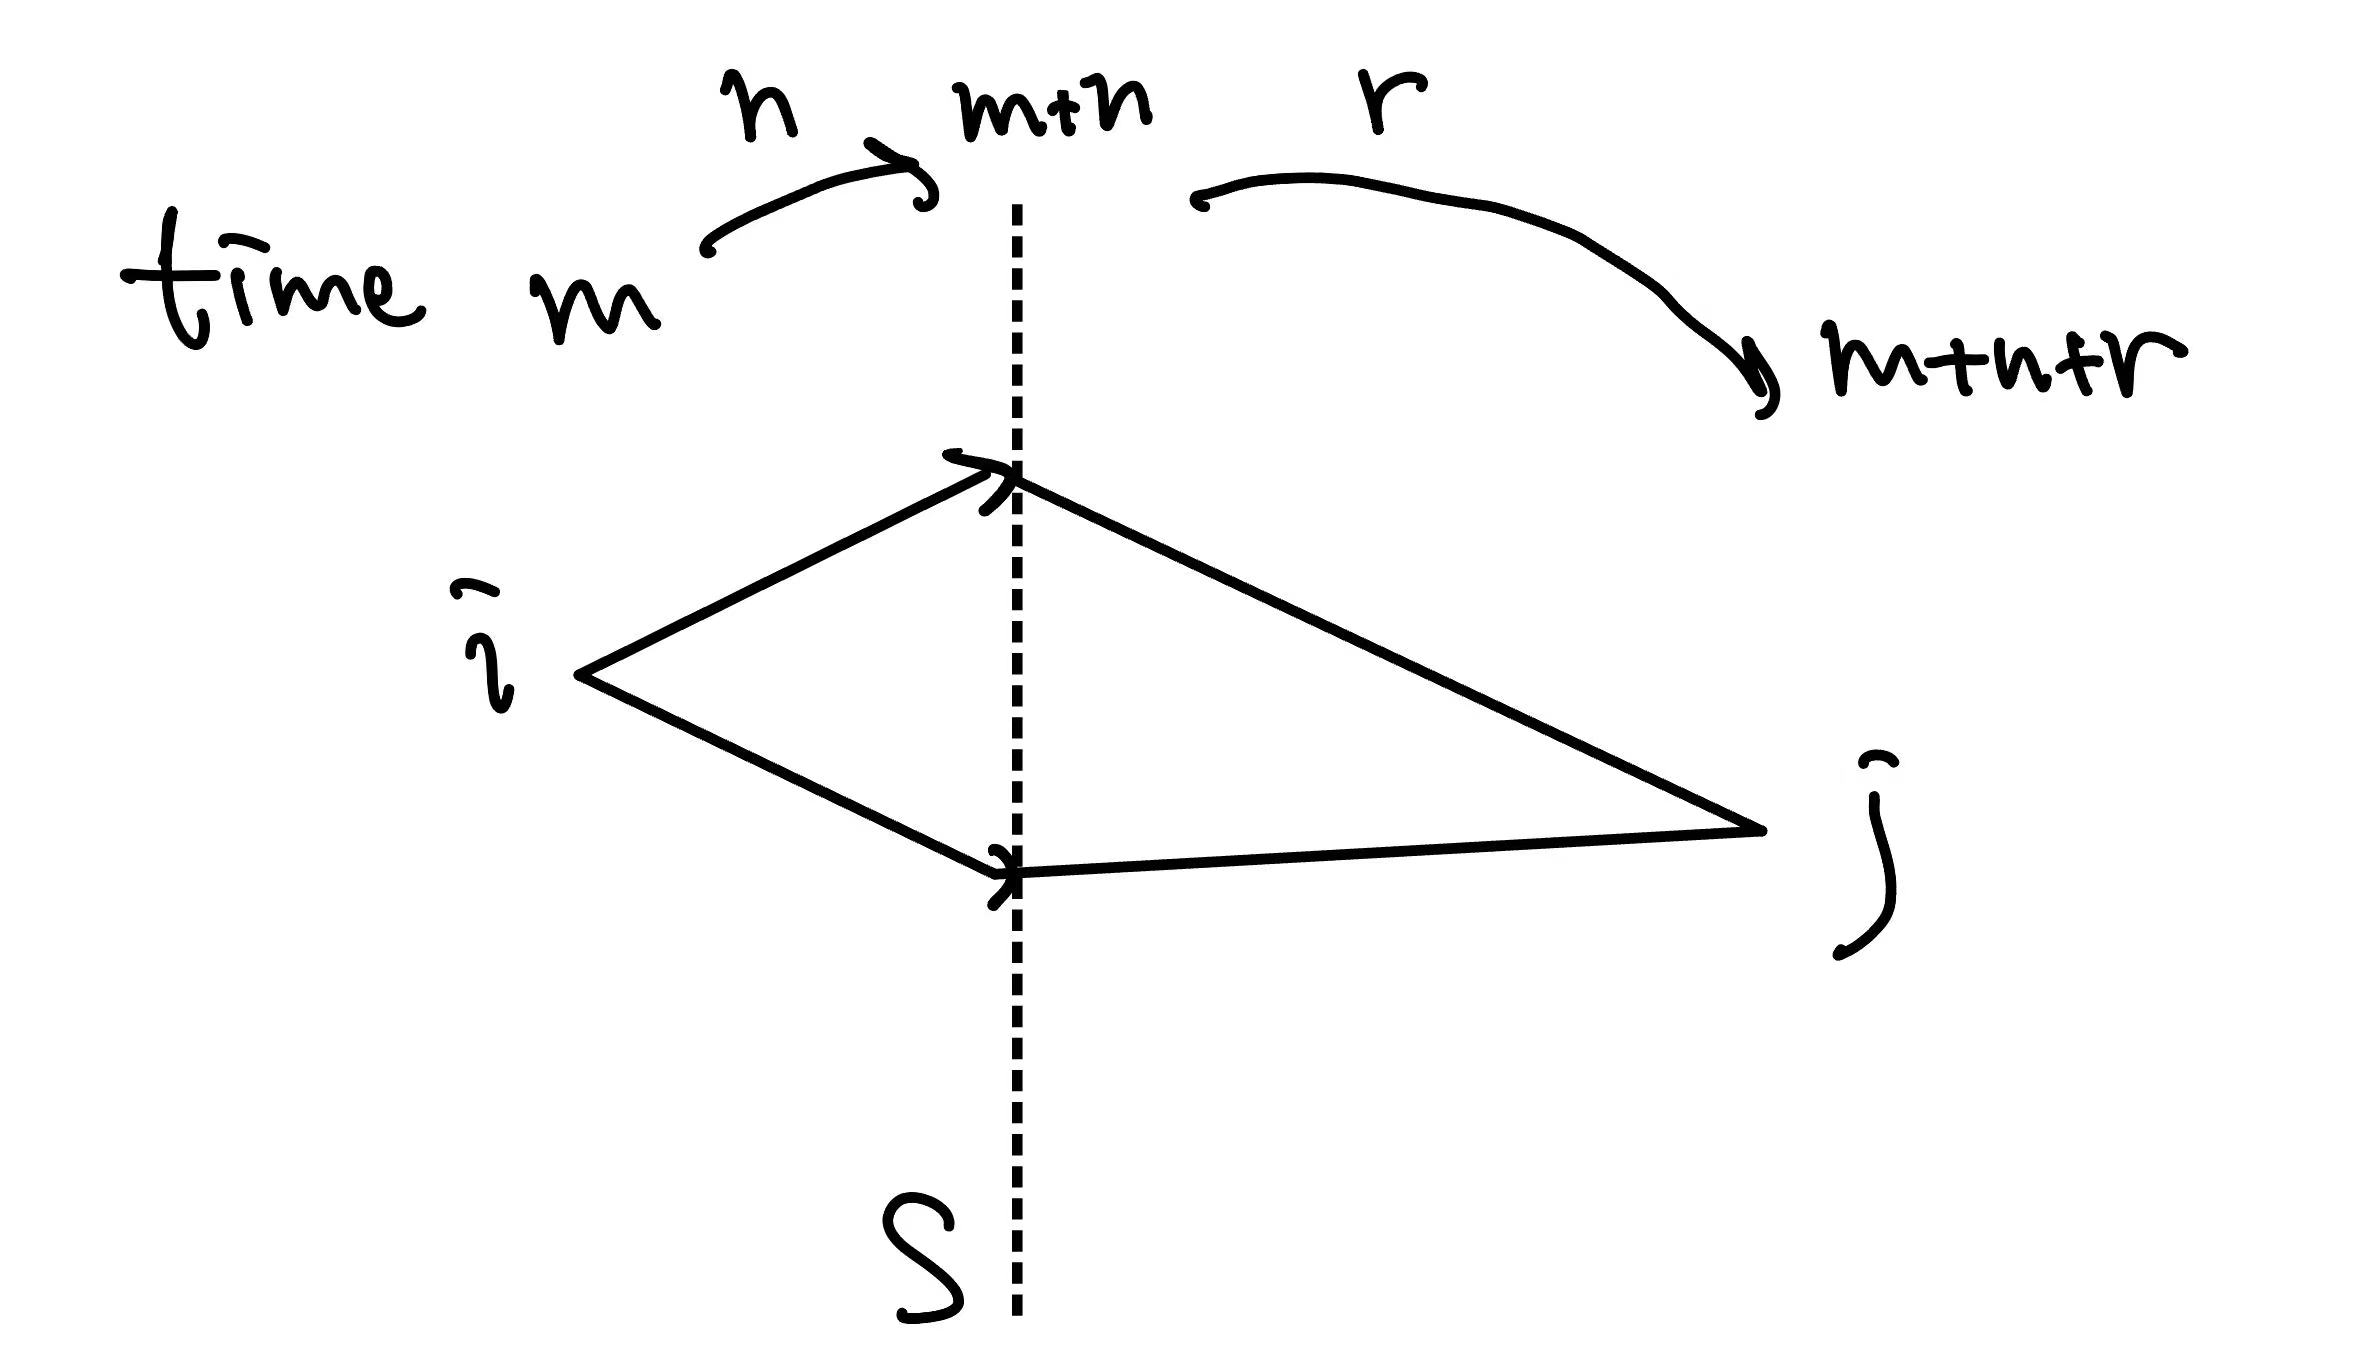
\includegraphics[width=0.55\textwidth]{figures/multi_steps.jpg}
    \caption{Multi-steps}
\end{figure}

证明:

\[
\begin{aligned}
    p_{ij}(m,m+n+r)&=P(X_{m+n+r}=j|X_m=i)\\
    &=\sum_{k\in S}P(X_{m+n+r}=j,X_{m+n}=k|X_m=i)\\
    &=\sum_{k\in S}\PP_{\{X_m=i\}}(X_{m+n+r}=j|X_{m+n}=k)\PP_{\{X_m=i\}}(X_{m+n}=k)\quad [\text{乘法公式}\eqref{eq:multiply_func}]\\
    &=\sum_{k\in S}p_{ik}(m,m+n)p_{kj}(m+n,m+n+r)\quad [\text{Markov}]
\end{aligned}
\]

\begin{corollary}
    设 $X$ 为具有(一步)转移矩阵 $P$ 的时齐马氏链, 则
    \begin{enumerate}
        \item $\forall m,n\geq 0$, 有 $P(m,m+n)=P(0,n)=P^n$.其中, 约定 $P^0=I$(单位矩阵)
        
        从而, 可记 $X$ 的 $n$ 步转移概率为 $p_{ij}(n)$ 或 $p_{ij}^{(n)}$, $n$ 步转移概率矩阵为 $P(n)$, 且有
        \[
        P(n)=P^n=(p_{ij}^{(n)})_{i,j\in S}
        \]
        \item C-K 方程可改写为
        \[
        p_{ij}(m+n)=\sum_{k\in S}p_{ik}^{(m)}p_{kj}^{(n)}
        \]
        $P(m+n)=P(m)P(n)$, 即 $P^{m+n}=P^m P^n$
    \end{enumerate}
\end{corollary}

证明:

\[
\begin{aligned}
    P(m,m+n)&=P(m,m+1)\cdot P(m+1,m+n)\quad [\text{C-K}]\\
    &=P\cdot P(m+1,m+n)\quad [\text{时齐}]\\
    &=P^n\qed
\end{aligned}
\]

\begin{proposition}
    $\forall n\geq 0, P(n)=P^n$ 仍是一个随机矩阵(定理\ref{thm:random_matrix})
\end{proposition}

证明:$n=2$时, $P^2=(p_{ij}(2))_{i,j\in S}$

$\Rightarrow$
\[
\begin{aligned}
    \sum_{j\in S}p_{ij}(2)&=\sum_{j\in S}\sum_{k\in S}p_{ik}p_{kj}\quad [\text{C-K}, \text{ 默认}p_{ik}(1)=p_{ik}]\\
    &=\sum_{k\in S}\sum_{j\in S}p_{ik}p_{kj}\\
    &=\sum_{k\in S}p_{ik}\cdot(\sum_{j\in S}p_{kj})\\
    &=\sum_{k\in S}p_{ik}=1\qed
\end{aligned}
\]
第二个等号, 级数可交换是因为非负, 要么有限(收敛)、要么$+\infty$(发散)

\subsubsection{马氏链的任意有限维分布}

\begin{proposition}
    $X\sim\text{Markov}(\mu, P)$, 其中 $\mu=(\mu_i)_{i\in S}, P=(p_{ij})_{i,j\in S}$, 则
    \[
    \PP(X_{u_1}=i_1,\cdots,X_{u_n}=i_n)=\mu_{i_1}^{(u_1)}\prod_{k=1}^{n-1}p_{i_k,i_{k+1}}^{(u_{k+1}-u_k)}
    \]
    其中, $0<u_1<u_2<\cdots<u_n$, $i_1,i_2,\cdots,i_n\in S$, $\mu^{(u_1)}=(\mu_i^{(u_1)})_{i\in S}$ 为 $X_{u_1}$ 的有限维分布
\end{proposition}

证明:
\[
\begin{aligned}
    \PP(X_{u_1}=i_1,\cdots,X_{u_n}=i_n)&=\PP(X_{u_1}=i_1)\cdot \PP(X_{u_2}=i_2|X_{u_1}=i_1)\cdots \PP(X_{u_n}=i_n|X_{u_1}=i_1,\cdots,X_{u_{n-1}}=i_{n-1})\\
    &=(\mu_{i_1}^{(u_1)})p_{i_1,i_2}^{(u_2-u_1)}\cdots p_{i_{n-1},i_n}^{(u_n-u_{n-1})}\quad [\text{Markov}]\\
    &=\mu_{i_1}^{(u_1)}\prod_{k=1}^{n-1}p_{i_k,i_{k+1}}^{(u_{k+1}-u_k)}
\end{aligned}
\]

用概率表示不够直观, 尝试用转移矩阵来表示

\begin{lemma}
   $\mu^{(m+n)}=\mu^{(n)}P^m(\forall m,n\geq 0)$, 即
   \[
   \mu_j^{(m+n)}=(\mu^{(n)}P^m)_j=\sum_{i\in S}\mu_i^{(n)}p_{ij}^{(m)}
   \]
   特别地, 取 $n=0$, 则 $\mu^{(m)}=\mu\cdot P^m$($\mu$看成行向量), 即 $\mu_j^{(m)}=(\mu P^m)_j=\sum_{i\in S}\mu_i\cdot p_{ij}^{(m)}$
\end{lemma}

证明:
\[
\begin{aligned}
    \mu_j^{(n+m)}=\PP(X_{n+m}=j)&=\sum_{i\in S}\PP(X_{n+m}=j|X_n=i)\PP(X_n=i)\\
    &=\sum_{i\in S}p_{ij}(m)\mu_i^{(n)}\\
    &=(\mu^{(n)}P^m)_j\qed
\end{aligned}
\]

$\Rightarrow \mu^{(m+n)}=\mu^{(n)}P^m$

\begin{theorem}[任意有限维分布II]
    $\forall 0\leq u_1<u_2<\cdots<u_n, i_1,\cdots,i_n\in S$
    \[
    \PP(X_{u_1}=i_1,\cdots,X_{u_n}=i_n)=(\mu P^{u_1}_{i_1})\prod_{k=1}^{n-1}P_{i_k,i_{k+1}}^{u_{k+1}-u_k}
    \]
    其中, $P_{i,j}^m=:(P^m)_{i,j}=:p_{i,j}^{(m)}$
\end{theorem}

讨论随机过程地存在性:

抽象地, $\mu,P\xrightarrow{\text{定理}\eqref{thm:Kolmogorov}}\text{有限维分布族}\rightarrow X\sim \text{Markov}(\mu,P)$, $\mu,P$可以刻画具备对称性、相容性的有限维分布

具体地, 参考Resnick\cite{resnick}, P62, Section 2.1

\newpage